\documentclass[11pt,oneside,a4paper]{book}

\usepackage{hyperref}
\usepackage{color}
%\usepackage{amssymb}
%Used for tildes urls
\usepackage{url}
%Used for longtables
\usepackage{longtable}
%Used for having noidentation for paragraphs
%and vertical spacing between them
\usepackage{parskip}
\usepackage{listings}
\usepackage{graphicx}
\usepackage{float}
	
\newcommand{\draft}[1]{\textcolor{blue}{#1}}
\newcommand{\hint}[1]{\textcolor{green}{[{\it#1}]}}
\newcommand{\fishy}[1]{\textcolor{red}{#1}}
\newcommand{\comment}[1]{\marginpar{\scriptsize{\textcolor{red}{#1}}}}
\newcommand{\mytilde}{\raise.17ex\hbox{$\scriptstyle\sim$}}
\newcommand{\mytildett}{\raise.17ex\hbox{$\scriptstyle\mathtt{\sim}$}}
\newenvironment{code}%
{
\addtolength{\leftskip}{0.5cm}}%
{

}

\begin{document}

\title{
\includegraphics[width=4cm]{images/Ptf_LogoBlau}\\ \vspace{1cm}
\textsf{\bf \huge PTF User's Guide}\\
       \normalsize PTF Version: 2.1}
\author{Michael Gerndt, Anamika Chowdhury}
\date{18.03.2016}

\maketitle

\tableofcontents

\chapter{Introduction}

Periscope is a scalable automatic performance tuning tool currently under development at Technical University of Munich and is part of the Periscope Tuning Framework (PTF), along with tools like Pathway and tuning plugins.

Periscope provides two main functionalities for Fortran and C/C++ applications: automatic \textit{performance tuning} and \textit{performance analysis}.

Performance tuning is provided through a set of tuning plugins. Periscope tuning plugins support aspect specific tuning. Each plugin uses expert knowledge to, for example, find the best configuration of the tuning parameters of the MPI library. Periscope offers the necessary support for measurements, search logic, and automatic execution of experiments for selected configurations. The best configuration is provided as an advice at the end of the tuning.

Automaric performance analysis is performed at runtime, using an iterative approach. There is a starting set of performance properties, which is then refined based on the measurements and the chosen search strategy. In the end, the appropriate set of performance properties is provided for the application being analyzed. The search threshold, the confidence value, and the severity are defined by means of a formal specification of the properties.

Based on expert knowledge, Periscope uses several strategies to identify possible performance issues. Such strategies provide profile information about program regions and performance properties for MPI and OpenMP.

Periscope consists of four main components: the \textit{frontend}, the \textit{hierarchy of communication and analysis agents}, and the \textit{monitoring library}.

\begin{itemize}
\item \textit{The frontend} is responsible for starting both the application to be analyzed, as well as all the internal components of Periscope. All settings regarding the execution of Periscope can be selected by means of command-line parameters of the frontend process. The frontend the loads the tuning plugins and executes the tuning.

\item The \textit{agent hierarchy} is transparent for the common users. At the bottom layer of the hierarchy there are the analysis agents. They control and configure the tuning actions and measurements for each application process. They can start, halt, or resume the application execution, and they also retrieve the performance data. Required tuning actions are communicated by the frontend and at the end of the local search, the tuning objective value is communicated back to the frontend and finally the tuning plugin.

\item The \textit{monitoring library} is also transparent to the user and it provides the measurement and communication layer between the application being tested and the performance tool. Periscope relies on the Score-P monitoring system.

\end{itemize}


\chapter{Quick Start}


\section{Installation}

\subsection{Access to pre-installed version}

PTF might have been already installed on your system. In order to use it, you have to add to your \texttt{.bashrc} file:

\begin{code}
\texttt{\$ module load periscope}
\end{code}

and then issue in your home directory:

\begin{code}
\texttt{\$ source .bashrc}
\end{code}

\textit{Note: Please make sure to add the command for loading the periscope module into your .bashrc. Just issuing the command at the command line is not going to work properly.}


If Periscope is not available as a module, it can be installed from the source files, following the common process of configuring and building using Autotools.

Please check the \textit{PTF Installation Manual} for a thorough guide on how to install Periscope on your machine.

\subsection{.periscope configuration file}

Before using Periscope, the \texttt{.periscope} setup file has to be created in your home directory. You may create a new one, or copy it from the Periscope installation directory:

\begin{code}
\texttt{\$ cp \$PSC\_ROOT/templates/.periscope \mytildett}
\end{code}


The setup file contains a list of \texttt{<option>=<value>} pairs, as follows:
\comment{Update}

\begin{code}
\texttt{MACHINE = SuperMUC\\
SITE = LRZ\\
REGSERVICE\_HOST = localhost\\
REGSERVICE\_PORT = 50001\\
REGSERVICE\_HOST\_INIT = localhost\\
REGSERVICE\_PORT\_INIT = 50001\\
APPL\_BASEPORT = 51000\\
AGENT\_BASEPORT = 50002}
\end{code}

If running on your local machine only, then the \texttt{MACHINE} option above should be set to \texttt{localhost}.

\begin{code}
\texttt{MACHINE = localhost}
\end{code}

Please refer to the \textit{PTF Periscope Installation Manual} for a detailed description on how to choose the proper option values for your particular system.

\subsection{SSH access}

In order to run Periscope, a private key based \texttt{ssh} access has to be provided on the machine running the tool. If not already configured, you can do so in few steps:

\begin{enumerate}
\item \texttt{\$ mkdir \mytilde/.ssh}
\item \texttt{\$ cd \mytilde/.ssh}
\item \texttt{\$ ssh-keygen -t rsa -N '' -f id\_rsa}
\item \texttt{\$ cat id\_rsa.pub \textgreater\textgreater\ authorized\_keys}
\item \texttt{\$ chmod 600 authorized\_keys}
\end{enumerate}

The \texttt{ssh} access is not required if running on your local machine, i.e. the \texttt{MACHINE} option is set to \texttt{localhost} in your \texttt{.periscope} file.


\section{First compiler flags tuning}

Having Periscope properly installed, there are only few steps required for tuning a test application:

\begin{enumerate}
	\item specify a \textit{phase region} by instrumenting the source code of the application with the Score-P pragma;
	\item modify the \texttt{Makefile} to enable instrumentation;
	\item build the application;
	\item start the tuning;
	\item inspect the tuning advice.
\end{enumerate}


For the remainder of this section we consider as the test application the NPB-MZ BT benchmark\footnote{See \url{http://www.nas.nasa.gov/publications/npb.html} for download and documentation.}. \comment{Make it a preconfigured test provided with PTF}

\subsection{Specify the phase region}

The PTF uses tuning plugins to determine candidate configurations for the tuning parameters of a plugin-specific tuning aspect. The search space is reduced by expert knowledge coded into the plugins. The configurations are then tested by running an experiment, and the objective value is measured. To not have to restart the application for each experiment, experiments make use of the iterative behavior of the application. Most scientific application do have a progress loop, and in each iteration a different configuration can be tested.

In order to do so, the repetitive region has to be marked in the source code as \textit{a phase region}. 

For the BT application, the phase region can be defined in file \texttt{bt.f}, lines 188 to 198, by inserting Score-p pragma as shown in Figure~\ref{fig:phase}.

\begin{figure}

\begin{lstlisting}[language=Fortran]

   SCOREP_USER_REGION_DEFINE(phase_handle )
   
c------------------------------------------------------
c   start the benchmark time step loop
c------------------------------------------------------

   do step = 1, niter
c----- lines omitted here ...

   SCOREP_USER_OA_PHASE_BEGIN(phase_handle, "PhaseRegion",
   SCOREP_USER_REGION_TYPE_COMMON)
   call exch_qbc(u,qbc,nx,nxmax,ny,nz)
		
   do zone = 1, num_zones
      call adi(rho_i(start1(zone)),us(start1(zone)),
     $         vs(start1(zone)),ws(start1(zone)),
     $         qs(start1(zone)),square(start1(zone)),
     $         rhs(start5(zone)),forcing(start5(zone)),
     $         u(start5(zone)),
     $         nx(zone),nxmax(zone),ny(zone),nz(zone))
   end do
   SCOREP_USER_OA_PHASE_END(phase_handle)
   end do
\end{lstlisting}
\caption{The phase region has to be marked with Score-P pragmas.}
\label{fig:phase}
\end{figure}

The file is already prepared for you in the test directory.
	
\subsection{Modify the makefile}

In order to enable performance measurements, the test application has to be instrumented by the performance tool. To enable instrumentation, one has to substitute the compile/link commands usually defined in the \texttt{Makefile}.

For NPB-MZ BT, one should edit the \texttt{config/make.def} file and update the \texttt{F77} variable as shown in Figure~\ref{fig:makefile}. This change was already done in the provided \texttt{make.def}.

\begin{figure}
\begin{code}
\texttt{\\
\#--------------------------------------------------------\\
\# This is the fortran compiler used for fortran programs\\
\#--------------------------------------------------------\\
F77=scorep --online-access --user ../bin/bt-mz.\$(CLASS).\$(NPROCS) -mpif77 \\
\# This links fortran programs; usually the same as \$(F77)\\
FLINK=\$(F77)\\
}
\end{code}
\caption{Enabling instrumentation of the phase region by Score-P in the makefile.}
\label{fig:makefile}
\end{figure}


\subsection{Build the application}

After the phase region was defined and the build command was adjusted, one can continue with the common build process of the test application.

For the NPB-MZ BT example, one should go to the root directory of the NPB-MZ series and issue:

\begin{code}
	\texttt{\\
	\$ make clean\\
	\$ make bt-mz CLASS=C NPROCS=16}
\end{code}

\subsection{Start compiler flags tuning}

Periscope can be started via its frontend \texttt{psc\_frontend}. Upon calling the executable with proper parameters, both Periscope's internal components as well as the test application are being started and the the tuning is carried out.

For the NPB-MZ BT example, one should go to the \texttt{bin} directory and then call \texttt{psc\_frontend} as follows:

\begin{code}
\texttt{\$ psc\_frontend --apprun=./bt-mz.C.16 --mpinumprocs=16 \\--tune=compilerflags --force-localhost}
\end{code}

This example demonstrates the tuning of compiler flags. It is setup for Intel FORTRAN compiler. Make sure to use the appropriate modules. The plugin reads a provided configuration file and explores different configuration of compiler flags. A detailed description of the tuning plugin is provided in \comment{Compiler flags plugin users guide.}.

\subsection{Explore the results}

Upon successful termination, Periscope generates an advice file. This is a standard XML file and could be opened using any text editor. Periscope provides a script to pretty print the result. \comment{Explain usage of python script}.

\section{First MPI analysis}

After having prepared the application for tuning, it can be used for performance analysis as well. Here, we will perform an automatic MPI analysis. 

For the NPB-MZ BT example, one should go to the \texttt{bin} directory and then call \texttt{psc\_frontend} as follows:

\begin{code}
\texttt{\$ psc\_frontend --apprun=./bt-mz.C.16 --mpinumprocs=16 \\--strategy=MPI --force-localhost}
\end{code}

Here the {\tt --strategy} option is used instead of {\tt --tune}. The results are provided in form of the found properties in the \texttt{properties\_*} file with the \texttt{.psc} extension. You can use the python script again to check the found performance properties.

\comment{Show usage of python script.}

\chapter{Preparing Applications}

\section{Specification of a phase region}\label{sec:phaseregion}

The performance measurements carried out within one \textbf{experiment} of the iterative analysis could be applied to either the entire application or only a particular execution \textit{phase} or code \textit{region}. Periscope offers the possibility to define such a \textbf{phase region} by means of manual instrumentation of the source code.

Please explore the Score-P user manual for the manual instrumentation in more detail. We only mention here that a phase region can be in terms of Periscope code instrumentation any regular user region.

A user region can be defined by inserting the following directives into the source code:\\
\textbf{Fortran:}\\
\begin{code}
program myProg\\
SCOREP\_USER\_REGION\_DEFINE( my\_region\_handle )\\
SCOREP\_USER\_REGION\_BEGIN( my\_region\_handle, "my\_region",\\ SCOREP\_USER\_REGION\_TYPE\_COMMON )\\
S1\\
S2\\
...\\
SCOREP\_USER\_REGION\_END( my\_region\_handle )\\
end program myProg
\end{code}

\textbf{C/C++:}\\
\begin{code}
void myfunc()\\
\{\\
SCOREP\_USER\_REGION\_DEFINE( my\_region\_handle )\\
SCOREP\_USER\_REGION\_BEGIN( my\_region\_handle, "my\_region",\\ SCOREP\_USER\_REGION\_TYPE\_COMMON )\\
S1\\
S2\\
...\\
SCOREP\_USER\_REGION\_END( my\_region\_handle )\\
\}
\end{code}

Periscope allows the specification of several \textit{user regions}, but only one such region can be defined as the \textbf{phase region}.

If several user regions are defined, but none of them is specified as the phase region, then the behaviour of Periscope is undefined.

If only one user region is specified, then this is automatically defined as the phase region.

If no phase region is specified, Periscope will automatically \textbf{restart the application} to perform new experiments, until no new candidate properties are found and the search terminates.

The use of phase regions is strongly recommended:
\begin{itemize}
	\item it reduces the overall execution time of the Periscope performance measurements;
	\item it delivers more accurate results, as measurements are only performed for relevant execution fragments.
\end{itemize}

The best example for a phase region is the body of the main loop of an application. It is common that scientific applications have a main loop iterating through time steps or grid elements. If such a \textit{repetitive region} is defined in the source code as a phase region, then the experiments can be done during the same application run. The application is suspended at the beginning of the phase region and new measurements are requested. The application is then released and the analysis is started. When the application encounters again the end of the region, it is suspended and the measured values are retrieved.


\section{Enabling instrumentation - \texttt{scorep}}

Measuring performance of an application is commonly based on the ability of the performance tool to "communicate" with the application at runtime. This can be achieved through the instrumentation of the application, i.e. inserting tool specific calls inside the source code or the compiled binary of the application. See also the right hand side of figure~\ref{fig:analysis-flow}.

In order to enable instrumentation with Score-P, one needs to \textit{prepend the compiling and linking commands} with the call to the \texttt{scorep} script. This could usually be done by editing the \texttt{Makefile} of the application.

For example, one should replace

\begin{code}
\texttt{mpif90 -c <args> }
\end{code}

with

\begin{code}
\texttt{scorep <scorep\_options> mpif90 -c <args>}
\end{code}

for a Fortran code, and

\begin{code}
\texttt{mpicc -c <args> }
\end{code}

with

\begin{code}
\texttt{scorep <scorep\_options> mpicc -c <args>}
\end{code}

for a C/C++ code.

Do not forget to change both the compiling \textbf{and} the linking commands.

Please note that the script recognizes the \texttt{-c} argument passed to the compiler itself and uses it to decide between the instrumentation and the linking steps. It is thus required that the respective test application is built in two distinct steps: compilation and linking.

The Score-P instrumenter command \texttt{scorep} automatically takes care of compilation and linking to produce an instrumented executable, and should be prefixed to
compile and link commands. Often this only requires prefixing definitions for CC
or MPICC (and equivalents) in Makefiles.

When compiling without the Score-P instrumenter, the \texttt{scorep-config} command can be used to simplify determining the appropriate linker flags and libraries, or include paths:

\texttt{scorep-config [--mpp=none|--mpp=mpi|--mpp=shmem]}\\
\texttt{ [--thread=none|--thread=omp|--thread=pthread] --libs}

Score-P supports a variety of instrumentation types for user-level source routines and arbitrary regions, in addition to fully-automatic MPI and OpenMP instrumentation, as summarized in Table
~\ref{table:instrumentation}. The detailed explanation can be found in Score-P user guide.

\begin{table}[H]
\centering
\begin{tabular}{|l|l|l|}
\hline
\begin{tabular}[c]{@{}l@{}}Type of \\ instrumen-\\ tation\end{tabular} & \begin{tabular}[c]{@{}l@{}}Instrumenter\\ switch\end{tabular} & \begin{tabular}[c]{@{}l@{}}Default \\ value\end{tabular}  \\ \hline
MPI & \begin{tabular}[c]{@{}l@{}}\texttt{--mpp=mpi/}\\ \texttt{--mpp=none} \end{tabular} & auto \\ \hline
SHMEM & \begin{tabular}[c]{@{}l@{}}\texttt{--mpp=shmem/}\\ \texttt{--mpp=none}\end{tabular} & auto  \\ \hline
OpenCL & \begin{tabular}[c]{@{}l@{}}\texttt{--opencl/}\\ \texttt{--noopencl}\end{tabular} & enabled  \\ \hline
OpenMP & \begin{tabular}[c]{@{}l@{}}\texttt{--thread=omp/}\\ \texttt{--thread=none}\end{tabular} & auto \\ \hline
Pthread & \begin{tabular}[c]{@{}l@{}}\texttt{--thread=pthread}\end{tabular} & auto \\ \hline
Compiler & \begin{tabular}[c]{@{}l@{}}\texttt{--compiler/}\\ \texttt{--nocompiler}\end{tabular} & enabled \\ \hline
PDT & \begin{tabular}[c]{@{}l@{}}\texttt{--pdt/}\\ \texttt{--nopdt}\end{tabular} & disabled \\ \hline
\begin{tabular}[c]{@{}l@{}}POMP2\\ user regions\end{tabular} & \begin{tabular}[c]{@{}l@{}} \texttt{--pomp/}\\ \texttt{--nopomp}\end{tabular} & \begin{tabular}[c]{@{}l@{}}depends \\ on\\ OpenMP\\ usage\end{tabular} \\ \hline
Manual & \begin{tabular}[c]{@{}l@{}}\texttt{--user/}\\ \texttt{--nouser}\end{tabular} & disabled \\ \hline
\end{tabular}
\label{table:instrumentation}
\end{table}


\chapter{Performance Tuning with Periscope}

Performance tuning using PTF (Periscope Tuning Framework) is based on the collaborative work performed by customized tuning plugins on the one side and Periscope as the host application of the plugins on the other side.

The high-level architecture of PTF can be seen in figure~\ref{fig:ptf-architecture}. Similar to using the analysis feature of PTF, users can start and configure the tuning process by calling the \texttt{psc\_frontend} with appropriate parameters. The option enabling the tuning execution mode of Periscope is \texttt{--tune}:

\begin{code}
\texttt{\$ psc\_frontend --tune=<nameofplugin> ...}
\end{code}

For example, the following will run compiler flags tuning (CFS) on the BT application:

\begin{code}
\texttt{psc\_frontend --apprun="./bt-MZ.W" --mpinumprocs=1 --force-localhost --tune=compilerflags --cfs-config="cfs\_config.cfg"}
\end{code}

Depending on each particular plugin, there might be also other options available for configuration. Please consult the corresponding \textit{User's Guide} for details specific to each of the plugins.

All other components in figure~\ref{fig:ptf-architecture} are transparent to the users of the plugins and of the PTF tuning feature.
\begin{figure}[bth]
	\centering
	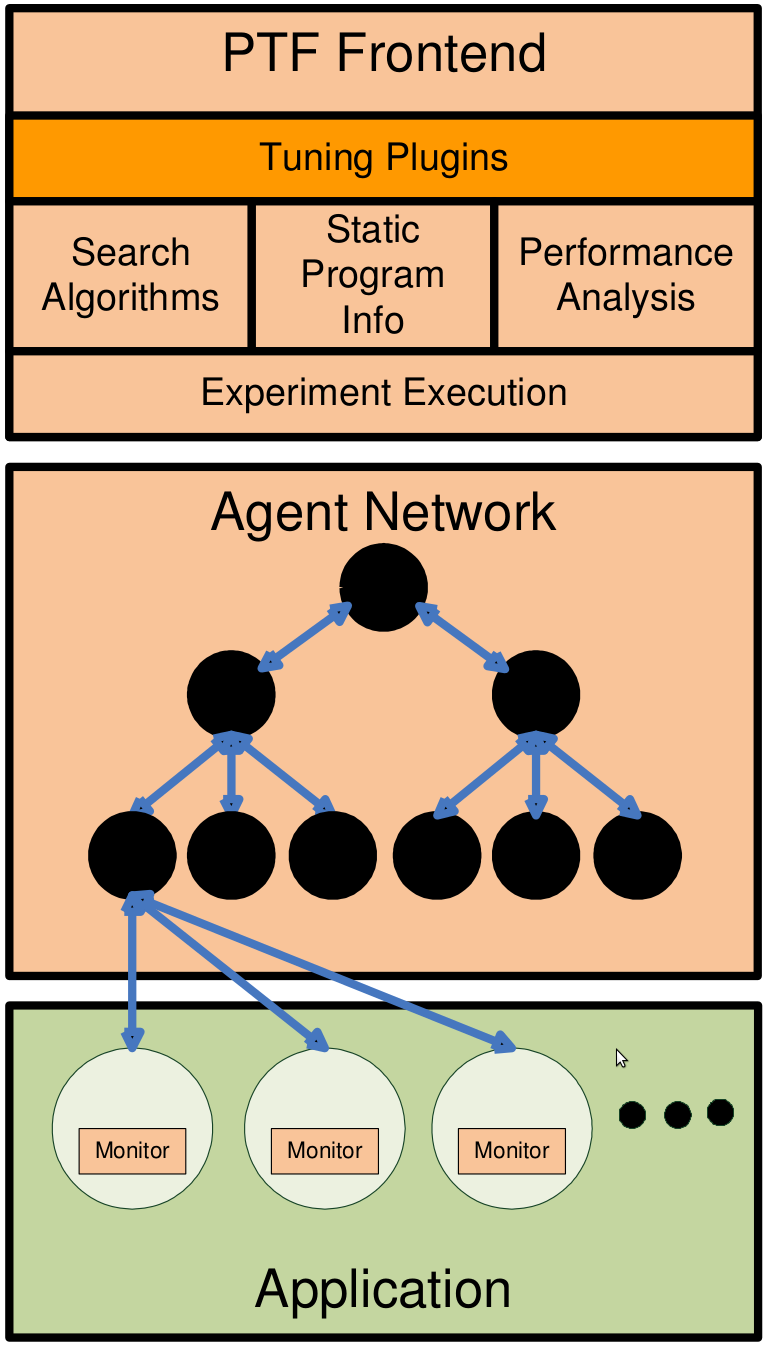
\includegraphics[width=.5\linewidth]{images/ptf-architecture}
	\caption{Plugin architecture of the Periscope Tuning Framework.}
	\label{fig:ptf-architecture}
\end{figure}


\section{Tuning plugins}
For the current version, PTF provides the following tuning plugins:

\begin{description}
\item[CFS:] the \textit{Compiler Flags Selection} plugin tunes the application to find the combination of compiler flags with which the best execution time is achieved.
\item[DVFS:] the \textit{Dynamic Voltage and Frequency Scaling} plugin tunes the energy consumption of an application.
\item[Master-Worker:] the \textit{Master-Worker} plugin tunes the number of tasks and processes to be used by applications based on the master-worker paradigm.
\item[MPI Paramenters:] automatically optimizes the values of a user selected subset of MPI configuration parameters.
\item[Patterns:] the \textit{Parallel Patterns} plugin works on applications using a \textit{Pipeline-based} execution to determine the best combination of the pipeline stages.
\end{description}


\section{Tuning advice}\label{sec:uninstrumented}
As a result of the tuning process, Periscope generates an XML file describing:

\begin{itemize}
	\item the final \textit{tuning advice} to be applied to the application
	\item the \textit{tuning scenarios} which were used in searching the best advice
	\item other information specific to the tuning plugin, like, for example, the tuning parameters, the execution times, or the energy consumption.
\end{itemize}

\section{The tuning flow}
Being the host of the tuning plugins, Periscope provides several services to build a standard tuning flow.

\subsection*{Data model}
The main components of the tuning data model are:

\begin{description}
	\item[tuning parameters:] represent the parameters based on which a tuning of the application can be done. These are plugin dependent and their semantics is strictly defined in each plugin. For example, the CFS plugin uses compiler flags as tuning parameters, while the MPI Parameters plugin uses MPI related switches and parameters.
	
	For most plugins, the tuning parameters are the given by user input through a configuration file.
	
	\item[tuning scenario:] represents a combination of tuning parameters. The application is analysed by Periscope using one scenario at a time.
	
	Scenarios are computed internally based on a chosen search algorithm. Users can choose between different search algorithms, but cannot directly define tuning scenarios.
	
	\item[tuning space:] the set of all valid tuning scenarios.
	\item[analysis result:] the analysis result associated with one specific tuning scenario. Results are partially displayed in the final tuning advice provided by Periscope.
\end{description}

\subsection*{Operations}
On the functional side, the tuning flow is supported by means two main operations:

\begin{description}
	\item[search algorithm:] the search algorithm generates the tuning space and  delivers the next scenario to be evaluated. For most tuning plugins, users can choose the preferred search algorithm.
	
	There are several search algorithms available: exhaustive search, individual search, random search and GDE3 search (one genetic algorithm).
	
	\item[pre-analysis:] some plugins require an analysis step before the tuning process can start. The Periscope performance analysis feature is being used in this case.
	
	Required pre-analysis is very much plugin specific. Please consult the given \textit{User's Guide} to see whether user input is possible for each particular case.
	
\end{description}



\section{Tuning uninstrumented applications}

The CFS Plugin an the MPI Plugin also allow tuning of uninstrumented applications, but this is strongly not encouraged. When measuring performance for uninstrumented applications, Periscope relies exclusively on the data retrieved from the system. This mostly leads to inaccuracies, especially for applications with a short execution time. If one does want to use the uninstrumented version, this can be done by passing the \texttt{--uninstrumented} option to the \texttt{psc\_frontend} process at the command line.



\chapter{Performance Analysis with Periscope}

Periscope follows an \textbf{iterative analysis} approach: it determines performance properties based on measurements, decides on possible new candidate properties and then it performs again new experiments to measure the data required to check whether the candidate properties hold. See also the cycle depicted in Figure~\ref{fig:analysis-flow}.

\begin{figure}[bth]
	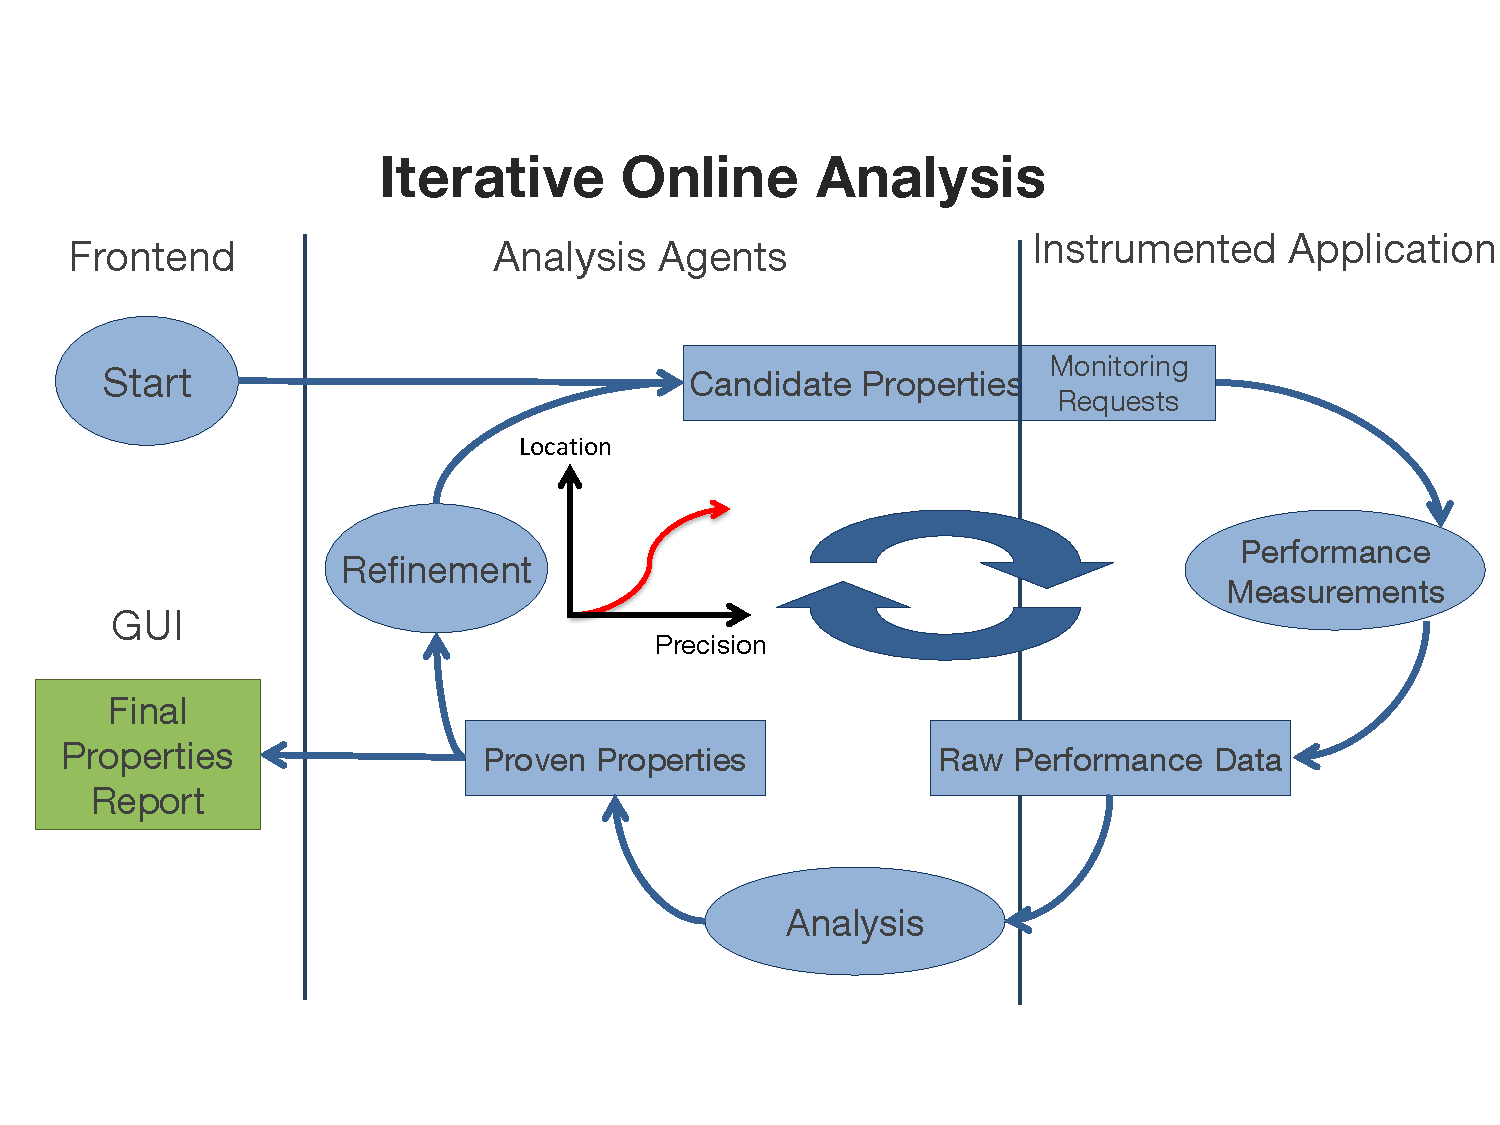
\includegraphics[width=\linewidth]{images/Periscope-iterative-analysis-slide}
	\caption{Periscope iterative analysis.}
	\label{fig:analysis-flow}
\end{figure}

The number of experiments carried out in one run of Periscope depends on both the execution time of the application itself and also the performance issues it might exhibit.

The number of experiments carried out in one run of Periscope depends on  the performance issues it might detect. Thus the total execution time of one Periscope analysis will depend on both the the execution time of the application itself, as well as the amount and severity of detected performance issues.


\section{Starting performance analysis - \texttt{psc\_frontend}}
The Periscope performance measurement and analysis process can be started via the \texttt{psc\_frontend} executable. For example:

\begin{code}
\texttt{\$ psc\_frontend --apprun=./bt-mz\_C.16 --mpinumprocs=16 \\--force-localhost --debug=1}
\end{code}

All needed configuration options can be passed to Periscope by means of the command line parameters.

The mandatory parameters which are required for Periscope analysis to start are:

\begin{center}
 \begin{longtable}{|l|p{6.5cm}|} % 3 cols (left, ctr, right); vert. lines
  \hline % draw horizontal line
  Option & Description \\
  \hline
  -{}-apprun=\textless command line\textgreater &
  Specify the command line to start the application. It will be passed to the mpirun command. \newline
  The executable specified in the command line must exist when Periscope is started. \\
  \hline
  -{}-mpinumprocs=\textless np\textgreater & Number of MPI processes for the
  application.\newline\newline
  For serial applications, please set this value to \texttt{1}. Periscope treats serial
  applications as 1-process MPI applications. \\
  \hline
 \end{longtable}
\end{center}

Other frequently used options are:
\begin{center}
 \begin{longtable}{|l|p{6.5cm}|} % 3 cols (left, ctr, right); vert. lines
  \hline % draw horizontal line
  Option & Description \\
  \hline
  -{}-debug=\textless level\textgreater & Level of debug output (default: 0). \\
  \hline
  -{}-force-localhost & Locally start the agents instead of using SSH. \\
  \hline
  -{}-strategy=\textless strategy\textgreater & Specify one of the following
  strategies: MPI, SCA, SCABF, P6, P6BF, P6BF\_Memory, SCPS\_BF,
  scalability\_OMP. Please note: Some strategies are platform dependent (default: all). \\
   \hline
  -{}-propfile=\textless filename\textgreater & Store the detected properties
  into filename (default: properties.psc) \\
  \hline
  -{}-ompnumthreads=\textless threads\textgreater & Number of OpenMP threads (default: 1).\\
  \hline
 \end{longtable}
\end{center}

Please see table~\ref{table:frontend-options} for a complete list of options accepted by \texttt{psc\_frontend}.

On startup, a hierarchy of analysis and communication agents is first created, then the application to be measured is started and the analysis agents attach to the application nodes. The performance data are gathered by means of the monitoring library and communicated to the low-level agents. There it is analysed using the strategy established at the beginning within the frontend and based on the results, the next step of the iterative analysis is established.

The final results are propagated through the agent hierarchy up to the frontend, which then stores them in the properties file.

The frontend is the control point of Periscope. Users can configure and direct the performance analysis process from here. The agent hierarchy and the monitoring library remain transparent to the common user.


\section{Exploring the results - \texttt{GUI}}\label{sec:GUI}

The frontend writes the found performance properties into a file called \texttt{properties\_*} with the \texttt{.psc} extension. This file is in XML format and can be opened with any off-the-shelf text editor or a spreadsheet application.

Periscope also offers a Graphical User Interface (GUI) for an enhanced visualisation and exploration of the analysis results. It is an Eclipse based plugin, featuring a multi-functional table for displaying and organizing the textual data. Following functionalities are available:
\begin{itemize}
\item multiple criteria sorting algorithm
\item complex categorization utility
\item searching engine using \textit{regular expressions}
\item filtering operations
\item direct navigation from the bottlenecks to their precise source location using the default IDE editor for that source file type (e.g. CDT/Photran editor).
\end{itemize}

An outline view for the instrumented code regions that were used in an experiment is also available. The information it shows is a combination of the standard intermediate representation of the analyzed application and the distribution of its bottlenecks. The main goals of the view are to assist the navigation in the source code and attract developer's attention to the most problematic code areas.

The multivariate statistical clustering is another key feature of the plug-in that enhances the scalability of the GUI and provides means of conducting Peta-scale performance analysis. It can effectively summarize the displayed information and identify a runtime behavior possibly hidden in the large amount of data.


\chapter{Configuration Options}

\section{Environment Variables}

\begin{center}
 \begin{longtable}{|p{4.5cm}|p{7.5cm}|} % 3 cols (left, ctr, right); vert. lines
  \hline % draw horizontal line
  Option & Description \\
  \hline
  PSC\_ROOT & Root directory of the Periscope installation. \\
  \hline
  PERISCOPE\_DEBUG & 0..2\newline
  0=quiet\newline
  1=startup, found properties in each search\newline
  2=candidate properties and found properties in each strategy step \\
  \hline
 \end{longtable}
\end{center}

\newpage
\section{The frontend - \texttt{psc\_frontend}}

The frontend starts up the application and the agent hierarchy.

\begin{center}
 \label{table:frontend-options}
 \begin{longtable}{|p{5cm}|p{7cm}|}
  \hline
  Option & Description \\
  \hline
  -{}-apprun=\textless appl cmdline\textgreater &
  This is the command line used to start the application. It should be the same as in \texttt{mpirun -np <procs> <appl cmdline>}.\newline\newline
  This value is also used to determine the name of the SIR file, when \texttt{--sir} is missing.\newline\newline
   The executable specified in the command line must exist when Periscope is started. This is true also for the cases where the tuning feature of Periscope is used in combination with plugins which by themselves re-build the application from its source files (e.g. the CFS plugin).\\
  \hline

  -{}-debug=level &
  Level of debugging. All debug output up to that level will be printed.\newline
Default: PERISCOPE\_DEBUG or 0 \\
  \hline

  -{}-selective-debug=list &
  Individual debugging level names separated by comma\\
  \hline

  -{}-delay=\textless n\textgreater &
  Number of phase executions that are skipped before the search is started. This is useful for applications that have a different behaviour at the beginning. \\
  \hline

   -{}-duration=\textless n\textgreater &
 Search delay in seconds of phase\\
  \hline

  -{}-dontcluster &
  Do not use online clustering for the detected bottlenecks.\\
  \hline

  -{}-force-localhost &
  Locally start the agents instead of using SSH. \\
  \hline

  -{}-help &
  Help information \\
  \hline

  -{}-maxcluster=\textless n\textgreater &
  Maximum number of MPI processes analyzed by a single analysis agent.\newline\newline
  It is not used on the Bluegene since the analysisagents are running on the IO nodes. All processes on the compute nodes of an IO nodes connect to its analysisagent.\newline\newline Default: 64 \\
  \hline

 -{}-maxfan=\textless n\textgreater &
  Determines the fan-out of the tree of high-level agents in interactive mode.\newline\newline
  Default: 4 \\
  \hline
  -{}-mpinumprocs=\textless n\textgreater &
  Number of MPI processes to be started. \\
  \hline

  -{}-nprops=\textless n\textgreater &
  Specifies the number of properties the frontend prints to standard output. Regardless of this value, all properties are output to the properties file.\newline\newline Default: 50. \\
  \hline

  -{}-ompnumthreads=\textless n\textgreater &
  Number of OMP threads to be started per MPI process. \newline\newline Default: 1.\\
  \hline

  -{}-pedantic &
  Shows all detected properties.\\
  \hline

  -{}-phase=\textless fileid:rfl\textgreater &
  Specifies the phase region via the fileid and the region first line number.\newline\newline
  If no phase region is specified, a user region is selected if at least one is given in the code. If multiple are given, it is undefined which is selected. If no user region is given, the main program is the user region and the  program will be restarted for each strategy step.\newline\newline
  If you mark the phase region via a user region and would like to use user regions also to guide analysis, you have to give the fileid and rfl for the phase region. \\
  \hline

  -{}-iterations=\textless n\textgreater &
  Specifies how many phase region executions constitute one phase.\newline\newline
  If a single execution of your phase region is too fast to perform any sensible measurements, you can combine multiple iterations into a single phase and measure for the whole duration of these n executions.\newline\newline
  The phase execution should take at least a couple of seconds to produce meaningful results. \\
  \hline

  -{}-propfile=\textless filename\textgreater &
  Specify the file to use when exporting the properties.\newline\newline Default: properties.psc \\
  \hline

  -{}-cfs-config=filename &
  Relative path to the CFS plugin configuration file \\
 \hline

  -{}-strategy=\textless strategyname\textgreater &
  Strategy used by analysisagent. Currently one of\newline
  MPI - MPI Communication analysis\newline
  OMP - OpenMP analysis\newline
  P6 - Power6 Analysis (only on Power6 machines)\newline
  P6BF - Power6 Breadth First (only on Power6 machines)\newline
  P6BF\_Memory - Power6 Memory Behavior Analysis (only on Power6machines)\newline
  SCPS\_BF - Generic memory analysis strategy\newline
  scalability\_OMP - Automatic OpenMP scalability analysis \\
  \hline

  -{}-timeout=\textless secs\textgreater &
  Timeout for startup of the agent hierarchy.\newline
  Default: varying depending on the number of processes \\
  \hline

  -{}-uninstrumented &
  \textbf{Autotuning only}: instructs Periscope to tune an uninstrumented
  application. Use with caution. See also Section~\ref{sec:uninstrumented}.\\
  \hline

  -{}-name &
  defines the name of the application\\
  \hline

  -{}-version &
  Displays the version of Periscope.\\
  \hline

  -{}-starter=name &
  Specifies resource manager name. E.g. Fast Interactive, Interactive, SLURM\\
  \hline

  -{}-statemachine-trace &
  Collects and prints state-machine transitions\\
  \hline

   -{}-registry=\textless host:port\textgreater &
   This option defines the address of the registry service\\
  \hline

   -{}-port=\textless n\textgreater &
  Local port number\\
  \hline

   -{}-maxthreads=\textless n\textgreater &
  Maximum number of threads assigned to a node agent\\
  \hline

   -{}-masterhost=\textless hostname\textgreater &
 Name of the host where the frontend starts\\
  \hline

   -{}-hlagenthosts=\textless list\textgreater &
  List with host names of HL agents, e.g. --hlagenthost=h1,h2,...\\
  \hline

  -{}-nodeagenthosts=\textless list\textgreater &
  List with host names of analysis agents, e.g. --nodeagenthosts=h1,h2,...\\
  \hline

  -{}-agenthostfile=\textless name\textgreater &
  File containing host configuration\\
  \hline

  -{}-manual &
  Run Periscope in manual mode\\
  \hline

  -{}-property=\textless name\textgreater &
  Name of a property to export\\
  \hline
 \end{longtable}
\end{center}

\chapter{Advanced user information - technical details}
The application and the agent network are started through the \texttt{psc\_frontend} process. First the set of available processors is analysed and based on this the mapping of application and analysis agent processes are determined. Both the application and the agent hierarchy are then started and a command is propagated from the frontend down to the analysis agents to start the search. The search is performed according to a search strategy selected when the frontend is started.

Each of the analysis agents, i.e. the nodes of the agent hierarchy, searches autonomously for inefficiencies in a subset of the application processes.

The application processes are linked with a monitoring system that provides the \textit{Monitoring Request Interface} (MRI). The agents attach to the monitor via sockets. The MRI allows the agent to configure the measurements, to start, to halt, to resume the execution, and to retrieve the performance data. The monitor currently only supports summary information.

At the end of the local search, the detected performance properties are reported back via the agent hierarchy to the frontend.

\section{Agent hierarchy}
The layout of the agent hierarchy can be controlled by the user by means of the specific parameters of the \texttt{psc\_frontend} executable:

\begin{description}
	\item[maxfan:] determines the fan-out of the tree of high-level agents. By default this is set to 4.
	\item[maxcluster:] gives the maximum number of MPI processes analysed by a single analysisagent. The default number is 64.
\end{description}

Further information on how the agents work within a specific run of PTF can be gathered by using the \texttt{--selective-debug} parameter of the same \texttt{psc\_frontend} executable:

\begin{code}
 \texttt{--selective-debug= \textless level1\textgreater,\textless level2\textgreater... }
\end{code}

with the following \textit{levels} being relevant for the agent hierarchy:
\begin{description}
	\item[AgentApplComm:] displays information regarding the communication between the agents and the application nodes.
	\item[AutotuneAgentStrategy:] displays information regarding the analysis strategy used in the analysis agent for tuning. To be used only when the tuning feature of PTF is being used.	
\end{description}

Other values for the \texttt{--selective-debug} parameter can be found in the \textit{PTF Developer's Guide}.

Using a proper layout of the agent hierarchy is very important especially when performing analysis and tuning of applications on large systems.

Please note that, if the \texttt{--force-localhost} option of the \texttt{psc\_frontend} executable is being used, then the entire agent hierarchy will be started on a single node. This is not recommended for applications using a large number of processes, as the communication between the agents and the application nodes would result in a bottleneck with a negative influence on the overall analysis time.


\chapter{Known Issues}
\begin{itemize}
 \item Automatic restart of the application does not work on the Bluegene. Make sure, you specify a user region that is executed repetitively.
 \item C instrumentation: The name of an OMP pragma should not occur again as a string in another context in this pragma, e.g., in a variable name.
 \item Measurements might be wrong in recursive algorithms.
 \item Multiple running instances of Periscope might not work on some systems.
\end{itemize}

\chapter*{Examples}

You can find one example with the adapted makefile in \verb|~|/Periscope/testcases/add.

\section*{Example on SuperMUC}

Periscope can be used in batch jobs.

Example batch script:\newline

\#@ wall\_clock\_limit = 00:30:00\\
\#@ job\_name = mytest\\
\#@ job\_type = MPICH\\
\#@ class = test\\
\#@ island\_count = 1\\
\#@ node = 1\\
\#@ total\_tasks = 1\\
\#@ node\_usage = not\_shared\\
\#@ initialdir = .\\
\#@ output = out.txt\\
\#@ error = out.txt\\
\#@ notification = never\\
\#@ queue\\
. /etc/profile\\
. /etc/profile.d/modules.sh\\

export OMP\_NUM\_THREADS=1\\
psc\_frontend --apprun=../add.exe --mpinumprocs=1 --tune=compilerflags --phase="mainRegion" --force-localhost

\end{document}
